% Supplementary Information for the manuscript.
% Compile separately (Overleaf: Menu -> Main document -> supplementary.tex), or: latexmk -pdf supplementary.tex
% All tables and figures are generated by scripts/make_paper_assets.py.
%
% Numbering is referenced from main.tex:
%   Tables  S1 data completeness | S2 processing | S3 GAT | S4 stability (full) | S5-S7 grids | S8 checkpoint rule | S9 GTV-only | S10 CNN seeds | S11 GAT as CNN
%           S9 clinical encoding | S10 reproducibility checklist
%   Figures S1 CV-fold ROC DM and OS

\documentclass[11pt]{article}
\usepackage[a4paper,top=1.8cm,bottom=2cm,left=1.5cm,right=1.5cm]{geometry}
\usepackage[T1]{fontenc}
\usepackage{lmodern}
\usepackage{graphicx}
\usepackage{booktabs}
\usepackage{amsmath,amssymb}
\usepackage{caption}
\usepackage{float}
\usepackage{xcolor}
\usepackage{algorithm}
\usepackage{algpseudocode}
\usepackage[hidelinks]{hyperref}

\graphicspath{{figures/}}
\providecommand{\botrule}{\bottomrule}
\newcommand{\method}{GRAFS-GAT}  % keep identical to main.tex
% generated by scripts/make_paper_assets.py -- do not edit
\newcommand{\allDM}{276}
\newcommand{\allEvDM}{27}
\newcommand{\allEvLR}{30}
\newcommand{\allEvOS}{44}
\newcommand{\allLR}{276}
\newcommand{\allOS}{164}
\newcommand{\annRetrainDMMax}{0.89}
\newcommand{\annRetrainDMMin}{0.87}
\newcommand{\attMax}{0.048}
\newcommand{\attMin}{0.047}
\newcommand{\attPid}{HN1792}
\newcommand{\attProb}{0.63}
\newcommand{\attUniform}{0.048}
\newcommand{\aucDMCVClinChosen}{0.66}
\newcommand{\aucDMCVClinClinRF}{0.82}
\newcommand{\aucDMCVClinRef}{0.72}
\newcommand{\aucDMCVImgChosen}{0.68}
\newcommand{\aucDMCVImgRF}{0.55}
\newcommand{\aucDMCVImgRef}{0.61}
\newcommand{\aucDMCohClinChosen}{0.73}
\newcommand{\aucDMCohClinClinRF}{0.78}
\newcommand{\aucDMCohClinRef}{0.77}
\newcommand{\aucDMCohImgChosen}{0.73}
\newcommand{\aucDMCohImgRF}{0.53}
\newcommand{\aucDMCohImgRef}{0.66}
\newcommand{\aucLRCVClinChosen}{0.66}
\newcommand{\aucLRCVClinClinRF}{0.58}
\newcommand{\aucLRCVClinRef}{0.66}
\newcommand{\aucLRCVImgChosen}{0.55}
\newcommand{\aucLRCVImgRF}{0.61}
\newcommand{\aucLRCVImgRef}{0.63}
\newcommand{\aucLRCohClinChosen}{0.54}
\newcommand{\aucLRCohClinClinRF}{0.54}
\newcommand{\aucLRCohClinRef}{0.47}
\newcommand{\aucLRCohImgChosen}{0.55}
\newcommand{\aucLRCohImgRF}{0.46}
\newcommand{\aucLRCohImgRef}{0.40}
\newcommand{\aucOSCVClinChosen}{0.66}
\newcommand{\aucOSCVClinClinRF}{0.70}
\newcommand{\aucOSCVClinRef}{0.65}
\newcommand{\aucOSCVImgChosen}{0.64}
\newcommand{\aucOSCVImgRF}{0.66}
\newcommand{\aucOSCVImgRef}{0.64}
\newcommand{\aucOSCohClinChosen}{0.64}
\newcommand{\aucOSCohClinClinRF}{0.66}
\newcommand{\aucOSCohClinRef}{0.64}
\newcommand{\aucOSCohImgChosen}{0.62}
\newcommand{\aucOSCohImgRF}{0.64}
\newcommand{\aucOSCohImgRef}{0.63}
\newcommand{\bootSpecDM}{0.62}
\newcommand{\bootSpecLR}{0.64}
\newcommand{\bootSpecOS}{0.48}
\newcommand{\ciDMCVClinChosen}{0.37--0.94}
\newcommand{\ciDMCVClinClinRF}{0.71--0.93}
\newcommand{\ciDMCVClinRef}{0.56--0.88}
\newcommand{\ciDMCVImgChosen}{0.40--0.92}
\newcommand{\ciDMCVImgRF}{0.25--0.83}
\newcommand{\ciDMCVImgRef}{0.36--0.78}
\newcommand{\ciDMCohClinChosen}{0.57--0.90}
\newcommand{\ciDMCohClinClinRF}{0.68--0.87}
\newcommand{\ciDMCohClinRef}{0.63--0.88}
\newcommand{\ciDMCohImgChosen}{0.55--0.91}
\newcommand{\ciDMCohImgRF}{0.25--0.79}
\newcommand{\ciDMCohImgRef}{0.52--0.79}
\newcommand{\ciLRCVClinChosen}{0.52--0.78}
\newcommand{\ciLRCVClinClinRF}{0.48--0.69}
\newcommand{\ciLRCVClinRef}{0.54--0.79}
\newcommand{\ciLRCVImgChosen}{0.43--0.67}
\newcommand{\ciLRCVImgRF}{0.48--0.74}
\newcommand{\ciLRCVImgRef}{0.50--0.75}
\newcommand{\ciLRCohClinChosen}{0.41--0.66}
\newcommand{\ciLRCohClinClinRF}{0.44--0.66}
\newcommand{\ciLRCohClinRef}{0.32--0.60}
\newcommand{\ciLRCohImgChosen}{0.43--0.67}
\newcommand{\ciLRCohImgRF}{0.34--0.59}
\newcommand{\ciLRCohImgRef}{0.25--0.53}
\newcommand{\ciOSCVClinChosen}{0.55--0.76}
\newcommand{\ciOSCVClinClinRF}{0.60--0.79}
\newcommand{\ciOSCVClinRef}{0.54--0.76}
\newcommand{\ciOSCVImgChosen}{0.53--0.74}
\newcommand{\ciOSCVImgRF}{0.56--0.77}
\newcommand{\ciOSCVImgRef}{0.53--0.75}
\newcommand{\ciOSCohClinChosen}{0.53--0.74}
\newcommand{\ciOSCohClinClinRF}{0.56--0.75}
\newcommand{\ciOSCohClinRef}{0.53--0.75}
\newcommand{\ciOSCohImgChosen}{0.52--0.72}
\newcommand{\ciOSCohImgRF}{0.54--0.74}
\newcommand{\ciOSCohImgRef}{0.52--0.73}
\newcommand{\cnnPctMax}{88}
\newcommand{\cnnPctMin}{28}
\newcommand{\cnnRetrainDMClinMax}{0.89}
\newcommand{\cnnRetrainDMClinMin}{0.87}
\newcommand{\cnnRetrainDMImgMax}{0.80}
\newcommand{\cnnRetrainDMImgMin}{0.76}
\newcommand{\eDMHNPET}{27}
\newcommand{\eDMMAASTRO}{7}
\newcommand{\eLRHNPET}{30}
\newcommand{\eLRMAASTRO}{30}
\newcommand{\eOSHNPET}{44}
\newcommand{\eOSMAASTRO}{45}
\newcommand{\ensGainAll}{0.03}
\newcommand{\ensGainDM}{0.05}
\newcommand{\ensGainLR}{0.02}
\newcommand{\ensGainOS}{0.02}
\newcommand{\ensGainPos}{77}
\newcommand{\foldDMClin}{0.62}
\newcommand{\foldDMImg}{0.68}
\newcommand{\foldLRClin}{0.62}
\newcommand{\foldLRImg}{0.54}
\newcommand{\foldOSClin}{0.65}
\newcommand{\foldOSImg}{0.63}
\newcommand{\foldRangeDMClin}{0.44--0.69}
\newcommand{\foldRangeDMImg}{0.64--0.77}
\newcommand{\foldRangeLRClin}{0.56--0.66}
\newcommand{\foldRangeLRImg}{0.46--0.60}
\newcommand{\foldRangeOSClin}{0.64--0.66}
\newcommand{\foldRangeOSImg}{0.62--0.64}
\newcommand{\gatMeanDMCV}{0.60}
\newcommand{\gatMeanDMCoh}{0.58}
\newcommand{\gatMeanLRCV}{0.58}
\newcommand{\gatMeanLRCoh}{0.50}
\newcommand{\gatMeanOSCV}{0.63}
\newcommand{\gatMeanOSCoh}{0.62}
\newcommand{\gatRfDMCV}{6/9}
\newcommand{\gatRfDMCoh}{3/9}
\newcommand{\gatRfLRCV}{3/9}
\newcommand{\gatRfLRCoh}{3/9}
\newcommand{\gatRfOSCV}{2/8}
\newcommand{\gatRfOSCoh}{5/8}
\newcommand{\gatRfSigDMCV}{0}
\newcommand{\gatRfSigDMCoh}{0}
\newcommand{\gatRfSigLRCV}{0}
\newcommand{\gatRfSigLRCoh}{1}
\newcommand{\gatRfSigOSCV}{0}
\newcommand{\gatRfSigOSCoh}{0}
\newcommand{\gfsBigCluster}{87}
\newcommand{\gfsEdges}{1,637}
\newcommand{\gfsHybComm}{12}
\newcommand{\gfsThr}{0.51}
\newcommand{\gfsTrainEv}{23}
\newcommand{\gfsTrainN}{220}
\newcommand{\gridAboveDM}{85}
\newcommand{\gridAboveLR}{81}
\newcommand{\gridAboveOS}{97}
\newcommand{\gridMaxDM}{0.79}
\newcommand{\gridMaxLR}{0.71}
\newcommand{\gridMaxOS}{0.69}
\newcommand{\gridMedDM}{0.63}
\newcommand{\gridMedLR}{0.58}
\newcommand{\gridMedOS}{0.65}
\newcommand{\gridMinDM}{0.18}
\newcommand{\gridMinLR}{0.39}
\newcommand{\gridMinOS}{0.43}
\newcommand{\gtvClsDMCVClin}{0.82}
\newcommand{\gtvClsDMCVImg}{0.70}
\newcommand{\gtvClsDMCohClin}{0.77}
\newcommand{\gtvClsDMCohImg}{0.70}
\newcommand{\gtvClsLRCVClin}{0.68}
\newcommand{\gtvClsLRCVImg}{0.58}
\newcommand{\gtvClsLRCohClin}{0.76}
\newcommand{\gtvClsLRCohImg}{0.65}
\newcommand{\gtvClsOSCVClin}{0.69}
\newcommand{\gtvClsOSCVImg}{0.62}
\newcommand{\gtvClsOSCohClin}{0.67}
\newcommand{\gtvClsOSCohImg}{0.65}
\newcommand{\gtvGatDMCVClin}{0.66}
\newcommand{\gtvGatDMCVImg}{0.65}
\newcommand{\gtvGatDMCohClin}{0.71}
\newcommand{\gtvGatDMCohImg}{0.68}
\newcommand{\gtvGatLRCVClin}{0.59}
\newcommand{\gtvGatLRCVImg}{0.57}
\newcommand{\gtvGatLRCohClin}{0.56}
\newcommand{\gtvGatLRCohImg}{0.48}
\newcommand{\gtvGatOSCVClin}{0.66}
\newcommand{\gtvGatOSCVImg}{0.64}
\newcommand{\gtvGatOSCohClin}{0.68}
\newcommand{\gtvGatOSCohImg}{0.64}
\newcommand{\gtvNcls}{453}
\newcommand{\gtvNgat}{24}
\newcommand{\gtvNpat}{431}
\newcommand{\gtvRefDMCVClin}{0.77}
\newcommand{\gtvRefDMCVImg}{0.73}
\newcommand{\gtvRefDMCohClin}{0.83}
\newcommand{\gtvRefDMCohImg}{0.73}
\newcommand{\gtvRefLRCVClin}{0.71}
\newcommand{\gtvRefLRCVImg}{0.66}
\newcommand{\gtvRefLRCohClin}{0.76}
\newcommand{\gtvRefLRCohImg}{0.34}
\newcommand{\gtvRefOSCVClin}{0.64}
\newcommand{\gtvRefOSCVImg}{0.66}
\newcommand{\gtvRefOSCohClin}{0.67}
\newcommand{\gtvRefOSCohImg}{0.66}
\newcommand{\gtvSubMax}{25}
\newcommand{\gtvSubMed}{24}
\newcommand{\gtvSubMin}{5}
\newcommand{\kunBorutaDM}{0.39}
\newcommand{\kunBorutaLR}{0.32}
\newcommand{\kunBorutaOS}{0.36}
\newcommand{\kunCCDM}{0.55}
\newcommand{\kunCCLR}{0.45}
\newcommand{\kunCCOS}{0.43}
\newcommand{\kunHybDM}{0.50}
\newcommand{\kunHybLR}{0.54}
\newcommand{\kunHybOS}{0.54}
\newcommand{\kunLassoDM}{0.16}
\newcommand{\kunLassoLR}{0.29}
\newcommand{\kunLassoOS}{0.22}
\newcommand{\kunMrmrDM}{0.38}
\newcommand{\kunMrmrLR}{0.32}
\newcommand{\kunMrmrOS}{0.41}
\newcommand{\kunRfeDM}{0.39}
\newcommand{\kunRfeLR}{0.31}
\newcommand{\kunRfeOS}{0.43}
\newcommand{\kunSpecDM}{0.84}
\newcommand{\kunSpecLR}{0.84}
\newcommand{\kunSpecOS}{0.71}
\newcommand{\meanClinDM}{0.62}
\newcommand{\meanClinLR}{0.59}
\newcommand{\meanClinOS}{0.65}
\newcommand{\meanImgDM}{0.59}
\newcommand{\meanImgLR}{0.54}
\newcommand{\meanImgOS}{0.62}
\newcommand{\msSavedDM}{4}
\newcommand{\msSavedLR}{26}
\newcommand{\msSavedOS}{20}
\newcommand{\msSpreadMax}{0.39}
\newcommand{\msSpreadMaxHi}{0.84}
\newcommand{\msSpreadMaxLo}{0.46}
\newcommand{\msSpreadMaxWhat}{DM, cohort split, imaging and clinical inputs, reference configuration}
\newcommand{\msSpreadMed}{0.07}
\newcommand{\nCHUM}{65}
\newcommand{\nCHUS}{100}
\newcommand{\nConfigDM}{144}
\newcommand{\nConfigLR}{144}
\newcommand{\nConfigOS}{128}
\newcommand{\nDMHNPET}{276}
\newcommand{\nDMMAASTRO}{109}
\newcommand{\nHGJ}{89}
\newcommand{\nHMR}{40}
\newcommand{\nHNPETclin}{298}
\newcommand{\nHNPETimg}{294}
\newcommand{\nLRHNPET}{276}
\newcommand{\nLRMAASTRO}{121}
\newcommand{\nOSHNPET}{164}
\newcommand{\nOSMAASTRO}{135}
\newcommand{\nSigDM}{8}
\newcommand{\nSigLR}{0}
\newcommand{\nSigOS}{0}
\newcommand{\rfMeanDMCV}{0.62}
\newcommand{\rfMeanDMCoh}{0.63}
\newcommand{\rfMeanLRCV}{0.59}
\newcommand{\rfMeanLRCoh}{0.53}
\newcommand{\rfMeanOSCV}{0.63}
\newcommand{\rfMeanOSCoh}{0.63}
\newcommand{\rhoStabDM}{0.23}
\newcommand{\rhoStabLR}{-0.92}
\newcommand{\rhoStabOS}{-0.74}
\newcommand{\rhoValDMCV}{0.13}
\newcommand{\rhoValDMCoh}{0.42}
\newcommand{\rhoValLRCV}{0.07}
\newcommand{\rhoValLRCoh}{0.59}
\newcommand{\rhoValOSCV}{0.26}
\newcommand{\rhoValOSCoh}{0.30}
\newcommand{\ruleChosenDMCohClin}{0.48}
\newcommand{\ruleChosenLRCohClin}{0.63}
\newcommand{\ruleRefMax}{0.05}
\newcommand{\ruleRefMed}{0.02}
\newcommand{\seedSdDM}{0.17}
\newcommand{\seedSdLR}{0.06}
\newcommand{\seedSdOS}{0.05}
\newcommand{\singleDMMax}{0.87}
\newcommand{\singleDMMin}{0.21}
\newcommand{\singleDMgeCNN}{0.3}
\newcommand{\singleLRMax}{0.78}
\newcommand{\singleLRMin}{0.32}
\newcommand{\singleOSMax}{0.73}
\newcommand{\singleOSMin}{0.29}
\newcommand{\topoDMradiomicknn}{0.64}
\newcommand{\topoDMradiomicstar}{0.63}
\newcommand{\topoDMspatialknn}{0.60}
\newcommand{\topoDMspatialstar}{0.57}
\newcommand{\topoLRradiomicknn}{0.57}
\newcommand{\topoLRradiomicstar}{0.57}
\newcommand{\topoLRspatialknn}{0.55}
\newcommand{\topoLRspatialstar}{0.56}
\newcommand{\topoOSradiomicknn}{0.64}
\newcommand{\topoOSradiomicstar}{0.64}
\newcommand{\topoOSspatialknn}{0.64}
\newcommand{\topoOSspatialstar}{0.62}
\newcommand{\topoPid}{HN1260}
\newcommand{\topoSlice}{82}
\newcommand{\valChosenLRCVImg}{0.66}
\newcommand{\valRefLRCohImg}{0.35}
\newcommand{\vcCfgMax}{37}
\newcommand{\vcCfgMin}{9}
\newcommand{\vcCfgMtMax}{50}
\newcommand{\vcFoldMax}{11}
\newcommand{\vcNmodels}{3{,}744}
\newcommand{\vcRatioMax}{8.7}
\newcommand{\vcRatioMin}{1.7}
\newcommand{\vcSeedMax}{83}
\newcommand{\vcSeedMin}{63}
\newcommand{\vcSeedMtMax}{77}
\newcommand{\vcSeedMtMin}{48}
\newcommand{\vcSelMax}{12}
\newcommand{\vcSelMin}{2}
\newcommand{\vcTopoMax}{8}


\renewcommand{\thetable}{S\arabic{table}}
\renewcommand{\thefigure}{S\arabic{figure}}
\renewcommand{\thealgorithm}{S\arabic{algorithm}}
\captionsetup{font=small,labelfont=bf}
\setlength{\parskip}{0.3em}
\setlength{\textfloatsep}{10pt plus 2pt minus 3pt}
\setlength{\floatsep}{8pt plus 2pt minus 2pt}
\renewcommand{\topfraction}{0.92}
\renewcommand{\textfraction}{0.06}
\renewcommand{\floatpagefraction}{0.85}
\setcounter{topnumber}{3}\setcounter{totalnumber}{5}

\title{\textbf{Supplementary Information}\\[6pt]
\large Reproducibility and external validity of graph-based feature selection in radiomic graph attention networks for outcome prediction in head and neck cancer}
\author{}
\date{}

\begin{document}
\maketitle
\tableofcontents
\bigskip

%% =========================================================================================
\section{Data provenance and endpoint definitions}

The development data are the four Canadian centres of the Head-Neck-PET-CT collection (CHUM, CHUS, HGJ and HMR), and the external test data are the HN1 collection from MAASTRO Clinic; both are distributed by The Cancer Imaging Archive. Outcomes for the Canadian centres were read from the file \texttt{INFOclinical\_HN\_Version2\_30may2018.xlsx}, ignoring its sheet of excluded patients, and outcomes for MAASTRO from the corresponding columns of the HN1 clinical file. All times are measured from diagnosis. For locoregional recurrence (LR) and distant metastasis (DM), the time is the time to the event when it occurred and otherwise the time to last follow-up; for overall survival (OS) it is the time to death or, for surviving patients, to last follow-up.

Binary labels follow Mateus et al. A label of one denotes an event within the horizon of 24 months (LR, DM) or 48 months (OS). A label of zero denotes event-free follow-up of at least the horizon, with later events counted as zero. Patients censored before the horizon were excluded from the analysis of that endpoint.

Images were taken from the complete TCIA release of Head-Neck-PET-CT (\nHNPETclin{} patients). For each patient, the CT series of the pretreatment PET/CT and the radiotherapy structure set registered to it were used (structure set \texttt{RTstructCTsimCTPETCT} where available, otherwise \texttt{RTstructCTsimPETPETCT}, which shares the frame of reference of the CT). The primary GTV was identified per patient from the structure names; when the primary tumour was split into several structures, their union was used. Because some structure sets reference PET slices, contours were rasterised from their physical coordinates onto the CT grid rather than through slice references. PET, dose, plan and the separate planning CT series were not used. Table~\ref{tab:missing} confirms that every eligible patient and event of the clinical file had a CT with a primary GTV. The MAASTRO cohort was complete with 137 patients.

\begin{table}[!htb]
\centering
\caption{Eligible patients and events in the Head-Neck-PET-CT clinical file, and those with CT and primary GTV used in this study.}\label{tab:missing}
\begin{tabular}{@{}lcccc@{}}
\toprule
Outcome & \multicolumn{2}{c}{All patients in clinical file} & \multicolumn{2}{c}{Patients with CT + GTV} \\
\cmidrule(lr){2-3}\cmidrule(lr){4-5}
 & Patients & Events & Patients & Events \\
\midrule
Locoregional recurrence (2 y) & 276 & 30 & 276 & 30 \\
Distant metastasis (2 y) & 276 & 27 & 276 & 27 \\
Overall survival (4 y) & 164 & 44 & 164 & 44 \\
\botrule
\end{tabular}

\end{table}

%% =========================================================================================
\section{Image processing and radiomic features}

Table~\ref{tab:preproc} lists the processing settings. The primary GTV was taken from the primary-tumour label of the segmentation; nodal GTVs were not used.

\begin{table}[!htb]
\centering\small
\caption{Pre-processing and feature-extraction settings.}\label{tab:preproc}
\begin{tabular}{@{}ll@{}}
\toprule
Step & Setting \\
\midrule
Resampling & 1\,mm isotropic; CT linear, mask nearest neighbour (SimpleITK) \\
Peritumoral region & GTV bounding box enlarged by 50\,mm in every direction; GTV voxels removed \\
Body mask & CT $>-500$\,HU, largest 3-D connected component, holes filled per slice; \\
 & peritumoral region restricted to the body \\
Supervoxels & SLIC-zero (scikit-image), target 100, connectivity enforced, \\
 & input CT clipped to $[-160, 240]$\,HU and scaled to [0,1]; supervoxels $<8$ voxels discarded \\
Feature extractor & PyRadiomics, original image, bin width 25\,HU, no normalisation \\
Feature classes & first order 18, GLCM 24, GLRLM 16, GLSZM 16, GLDM 14, NGTDM 5 (total 93) \\
Regions & GTV and every supervoxel \\
\botrule
\end{tabular}
\end{table}

%% =========================================================================================
\section{Network, training and baselines}

Table~\ref{tab:gat} gives the network and training settings. The hyper-parameters follow those previously published for spatial radiomic graphs in head and neck cancer (Bae et al., Radiology: Imaging Cancer 2025), and OS uses the LR settings because no OS model had been specified. The random-forest baselines used 100 trees with a maximum depth of 10 and min--max scaling fitted on the training patients. Their resampling strategy (under-, over- or intermediate sampling) was chosen on validation AUC, and their decision threshold by the maximum Youden index on validation.

\begin{table}[!htb]
\centering\small
\caption{\method{} hyper-parameters and training settings.}\label{tab:gat}
\begin{tabular}{@{}lcc@{}}
\toprule
 & LR and OS & DM \\
\midrule
GAT layers & 5 & 3 \\
Hidden units per head / heads & 16 / 4 & 8 / 4 \\
Dropout (GAT layers) & 0.67 & 0.89 \\
Learning rate & $4\times10^{-4}$ & $3\times10^{-4}$ \\
Weight decay & $7\times10^{-4}$ & $8\times10^{-4}$ \\
Warm-up epochs & 10 & 5 \\
Class resampling per epoch & both classes to mean size & minority oversampling \\
Batch size & 64 & 64 \\
Trainable parameters (with clinical input) & 15,057 & 1,841 \\
\midrule
Read-out & \multicolumn{2}{c}{GTV node embedding, dropout 0.5, [+ 16 clinical variables], linear layer} \\
Loss / optimiser & \multicolumn{2}{c}{binary cross-entropy / Adam} \\
Scheduler & \multicolumn{2}{c}{linear warm-up, then ReduceLROnPlateau (patience 20, factor 0.5, minimum $10^{-5}$)} \\
Stopping & \multicolumn{2}{c}{early stopping on validation loss (patience 50), maximum 500 epochs} \\
Gradient clipping & \multicolumn{2}{c}{norm 1.0} \\
Checkpoint (primary) & \multicolumn{2}{c}{lowest validation loss (after epoch 10)} \\
Checkpoint (sensitivity) & \multicolumn{2}{c}{rule of Mateus et al.\ (Supplementary Section~\ref{sec:epoch}); maximum 200 epochs} \\
Seeds & \multicolumn{2}{c}{42, 43 and 44; probabilities averaged} \\
\botrule
\end{tabular}
\end{table}

%% =========================================================================================
\section{Feature-selection algorithms and stability}

Every selector receives the GTV features of the training patients of one split, that is, one CV fold or the cohort-split training set. It returns a ranking of all features, the first $k=6$ of which are used as node features. Before selection, non-finite values are imputed with the median, features with a standard deviation of at most $10^{-8}$ are removed, a signed $\log(1+|x|)$ transform is applied to features with absolute skewness above 2, and all features are z-scored.

The Graph-FS feature graph is built from the matrix $R$ of absolute Pearson correlations. An edge $(i,j)$ exists if $R_{ij} > \bar r + \alpha s_r$, where $\bar r$ and $s_r$ are the mean and standard deviation of the off-diagonal entries and $\alpha=0.3$. A feature without edges is connected to its most correlated feature. Algorithms~\ref{alg:cc}--\ref{alg:hyb} specify the three Graph-FS variants.

\begin{algorithm}[H]
\caption{Graph-FS, connected components (CC)}\label{alg:cc}
\begin{algorithmic}[1]
\State $\alpha \gets 0.3$
\Repeat
  \State build the feature graph with threshold $\bar r+\alpha s_r$ and find its connected components
  \State $\alpha \gets \alpha + 0.1$
\Until{the number of components is at least $k$ or $\alpha$ reaches its maximum}
\State in each component select the feature with the highest degree centrality
\State rank the representatives by component size and keep the first $k$
\end{algorithmic}
\end{algorithm}

\begin{algorithm}[H]
\caption{Graph-FS, spectral}\label{alg:spec}
\begin{algorithmic}[1]
\State build the feature graph with $\alpha=0.3$ and its Laplacian $L \gets D - A$
\State $U \gets$ eigenvectors of $L$ belonging to the $k$ smallest eigenvalues
\State cluster the rows of $U$ into $k$ groups with $k$-means
\State in each cluster select the feature closest to the cluster centroid
\end{algorithmic}
\end{algorithm}

\begin{algorithm}[H]
\caption{Graph-FS, hybrid (graph-guided relevance, introduced in this study)}\label{alg:hyb}
\begin{algorithmic}[1]
\State build the feature graph with $\alpha=0.3$ and its Laplacian $L \gets D - A$
\State $g \gets$ position of the largest gap among the 20 smallest eigenvalues of $L$
\State $C \gets \max(2k, g)$; partition the features into $C$ communities by spectral clustering
\State $F_j \gets$ ANOVA $F$ statistic of feature $j$ against the outcome in the training patients
\State in each community keep the feature with the largest $F$
\State retain the $k$ representatives with the largest $F$ (at most one per community)
\end{algorithmic}
\end{algorithm}

The supervised selectors were configured as follows. mRMR uses the FCQ criterion, with relevance given by the ANOVA $F$ statistic and redundancy by the mean absolute correlation with features already selected, applied greedily. LASSO is an L1-penalised logistic regression (liblinear solver, balanced class weights) with 25 values of the inverse penalty between $10^{-2.5}$ and 10 chosen by inner stratified cross-validated AUC; features are ranked by their entry point on the regularisation path and then by the magnitude of their coefficient. Boruta uses a random forest of 300 trees with depth 6 and balanced subsampling, 60 iterations and two-sided binomial tests with Bonferroni correction at $\alpha=0.05$; features are ranked by decision, number of hits and mean importance. RFE-RF removes 5\% of the features per step using a random forest of 200 trees with depth 6.

For two subsets $A$ and $B$ of size $k$ drawn from $p$ features with overlap $r=|A\cap B|$, the Kuncheva index is $(rp-k^2)/\{k(p-k)\}$ and the Jaccard index is $|A\cap B|/|A\cup B|$. Kendall's $W$ measures the concordance of the complete rankings, and the core-80 fraction is the proportion of selected features that are chosen in at least 80\% of the runs. Table~\ref{tab:stabfull} reports these measures for every strategy, endpoint and setting.

\begin{table}[!htb]
\centering
\caption{Feature-selection stability: Jaccard index (J), Kendall's $W$ (W) and core-80 fraction (C80) for every strategy and setting (5-fold CV design).}\label{tab:stabfull}
\resizebox{\textwidth}{!}{\begin{tabular}{@{}llccccccccc@{}}
\toprule
 & & \multicolumn{3}{c}{Across CV folds} & \multicolumn{3}{c}{Bootstrap} & \multicolumn{3}{c}{Across centres} \\
\cmidrule(lr){3-5}\cmidrule(lr){6-8}\cmidrule(lr){9-11}
Outcome & Method & J & W & C80 & J & W & C80 & J & W & C80 \\
\midrule
LR & mRMR & 0.23 & 0.63 & 0.33 & 0.14 & 0.28 & 0.03 & 0.06 & 0.28 & 0.00 \\
 & LASSO & 0.22 & 0.62 & 0.33 & 0.13 & 0.37 & 0.00 & 0.06 & 0.49 & 0.00 \\
 & Boruta & 0.23 & 0.59 & 0.17 & 0.12 & 0.28 & 0.00 & 0.05 & 0.28 & 0.00 \\
 & RFE-RF & 0.22 & 0.54 & 0.17 & 0.10 & 0.28 & 0.00 & 0.05 & 0.31 & 0.00 \\
 & Graph-FS (CC) & 0.34 & 0.70 & 0.50 & 0.24 & 0.43 & 0.03 & 0.09 & 0.34 & 0.00 \\
 & Graph-FS (spectral) & 0.74 & 0.73 & 0.83 & 0.51 & 0.47 & 0.67 & 0.14 & 0.34 & 0.00 \\
 & Graph-FS (hybrid) & 0.40 & 0.69 & 0.67 & 0.20 & 0.39 & 0.10 & 0.10 & 0.35 & 0.00 \\
\midrule
DM & mRMR & 0.27 & 0.86 & 0.17 & 0.27 & 0.64 & 0.17 & 0.09 & 0.49 & 0.03 \\
 & LASSO & 0.13 & 0.58 & 0.00 & 0.14 & 0.46 & 0.00 & 0.09 & 0.61 & 0.03 \\
 & Boruta & 0.29 & 0.86 & 0.33 & 0.27 & 0.64 & 0.13 & 0.10 & 0.55 & 0.03 \\
 & RFE-RF & 0.29 & 0.78 & 0.33 & 0.25 & 0.57 & 0.13 & 0.08 & 0.46 & 0.00 \\
 & Graph-FS (CC) & 0.43 & 0.69 & 0.50 & 0.25 & 0.47 & 0.00 & 0.10 & 0.49 & 0.03 \\
 & Graph-FS (spectral) & 0.74 & 0.91 & 0.83 & 0.49 & 0.47 & 0.70 & 0.19 & 0.40 & 0.13 \\
 & Graph-FS (hybrid) & 0.37 & 0.90 & 0.50 & 0.29 & 0.70 & 0.17 & 0.11 & 0.54 & 0.00 \\
\midrule
OS & mRMR & 0.30 & 0.86 & 0.50 & 0.17 & 0.49 & 0.03 & 0.05 & 0.33 & 0.00 \\
 & LASSO & 0.16 & 0.59 & 0.17 & 0.12 & 0.40 & 0.00 & 0.06 & 0.52 & 0.00 \\
 & Boruta & 0.26 & 0.76 & 0.33 & 0.15 & 0.36 & 0.03 & 0.03 & 0.32 & 0.00 \\
 & RFE-RF & 0.31 & 0.58 & 0.33 & 0.12 & 0.29 & 0.00 & 0.05 & 0.31 & 0.00 \\
 & Graph-FS (CC) & 0.32 & 0.76 & 0.33 & 0.22 & 0.49 & 0.03 & 0.07 & 0.36 & 0.00 \\
 & Graph-FS (spectral) & 0.59 & 0.70 & 0.67 & 0.36 & 0.36 & 0.23 & 0.13 & 0.25 & 0.00 \\
 & Graph-FS (hybrid) & 0.40 & 0.89 & 0.67 & 0.20 & 0.57 & 0.03 & 0.08 & 0.39 & 0.00 \\
\botrule
\end{tabular}
}
\end{table}

%% =========================================================================================
\section{External AUC of every configuration}

Tables~\ref{tab:gridLR}--\ref{tab:gridOS} give the external (MAASTRO) AUC of every GAT configuration under the primary checkpoint rule; in the cross-validation design these are fold- and seed-ensemble AUCs. Bootstrap confidence intervals, validation AUCs, DeLong $p$ values and stability indices of every configuration are provided in the file \texttt{all\_configurations.csv}.

\newcommand{\gridblock}[2]{\par\smallskip\noindent\textit{#1}\par\smallskip{\small\input{tables/#2}}\par}

\begin{table}[!htb]
\centering
\caption{Locoregional recurrence: external AUC by feature-selection strategy and topology.}\label{tab:gridLR}
\gridblock{5-fold CV, imaging}{tabS_grid_LR_cv_img}
\gridblock{5-fold CV, imaging and clinical}{tabS_grid_LR_cv_clin}
\gridblock{Cohort split, imaging}{tabS_grid_LR_coh_img}
\gridblock{Cohort split, imaging and clinical}{tabS_grid_LR_coh_clin}
\end{table}

\begin{table}[!htb]
\centering
\caption{Distant metastasis: external AUC by feature-selection strategy and topology.}\label{tab:gridDM}
\gridblock{5-fold CV, imaging}{tabS_grid_DM_cv_img}
\gridblock{5-fold CV, imaging and clinical}{tabS_grid_DM_cv_clin}
\gridblock{Cohort split, imaging}{tabS_grid_DM_coh_img}
\gridblock{Cohort split, imaging and clinical}{tabS_grid_DM_coh_clin}
\end{table}

\begin{table}[!htb]
\centering
\caption{Overall survival: external AUC by feature-selection strategy and topology (no published feature set exists for OS).}\label{tab:gridOS}
\gridblock{5-fold CV, imaging}{tabS_grid_OS_cv_img}
\gridblock{5-fold CV, imaging and clinical}{tabS_grid_OS_cv_clin}
\gridblock{Cohort split, imaging}{tabS_grid_OS_coh_img}
\gridblock{Cohort split, imaging and clinical}{tabS_grid_OS_coh_clin}
\end{table}

%% =========================================================================================
\section{Checkpoint-rule sensitivity analysis}\label{sec:epoch}

Table~\ref{tab:epoch} compares the primary checkpoint rule (lowest validation loss) with the checkpoint rule of Mateus et al., implemented as in their published code, and with an adapted variant used in an earlier version of this analysis. Under the original rule a checkpoint is saved whenever the validation AUC exceeds both the best saved value and an endpoint-specific threshold while the training and validation AUCs differ by less than a set margin (DM 0.80/0.03, with clinical variables 0.80/0.05; LR 0.70/0.03 and 0.65/0.15; OS 0.75/0.05 and 0.70/0.05); the last saved checkpoint is retained, training stops when the training AUC exceeds 0.95, and the final epoch is used if nothing was saved. A checkpoint was saved in only \msSavedDM\% of DM, \msSavedLR\% of LR and \msSavedOS\% of OS networks. The adapted variant selects the highest validation AUC among epochs with a training--validation gap of at most 0.05, relaxing the gap in steps of 0.05 until an epoch qualifies. Because the configuration chosen on validation can change with the rule, the reference configuration provides the cleaner comparison; its external AUC changed by a median of \ruleRefMed{} and at most \ruleRefMax.

\begin{table}[!htb]
\centering
\caption{External AUC [95\% CI] of the chosen and reference GATs under the three checkpoint rules.}\label{tab:epoch}
\resizebox{\textwidth}{!}{\begin{tabular}{@{}llllccc@{}}
\toprule
Outcome & Design & Inputs & Model & Lowest val.\ loss & Mateus et al.\ rule & Adapted AUC-gap rule \\
\midrule
LR & 5-fold CV & Img & chosen & 0.55 [0.43, 0.67] & 0.55 [0.43, 0.67] & 0.60 [0.48, 0.73] \\
 & 5-fold CV & Img & reference & 0.63 [0.50, 0.75] & 0.63 [0.51, 0.75] & 0.63 [0.51, 0.76] \\
 & 5-fold CV & Img+Clin & chosen & 0.66 [0.52, 0.78] & 0.58 [0.47, 0.69] & 0.66 [0.53, 0.78] \\
 & 5-fold CV & Img+Clin & reference & 0.66 [0.54, 0.79] & 0.68 [0.55, 0.79] & 0.65 [0.52, 0.76] \\
 & Cohort split & Img & chosen & 0.55 [0.43, 0.67] & 0.57 [0.45, 0.68] & 0.56 [0.45, 0.69] \\
 & Cohort split & Img & reference & 0.40 [0.25, 0.53] & 0.44 [0.29, 0.58] & 0.44 [0.29, 0.56] \\
 & Cohort split & Img+Clin & chosen & 0.54 [0.41, 0.66] & 0.63 [0.51, 0.73] & 0.66 [0.55, 0.76] \\
 & Cohort split & Img+Clin & reference & 0.47 [0.32, 0.60] & 0.50 [0.34, 0.63] & 0.49 [0.35, 0.60] \\
\midrule
DM & 5-fold CV & Img & chosen & 0.68 [0.40, 0.92] & 0.64 [0.32, 0.93] & 0.63 [0.30, 0.93] \\
 & 5-fold CV & Img & reference & 0.61 [0.36, 0.78] & 0.66 [0.47, 0.81] & 0.64 [0.44, 0.79] \\
 & 5-fold CV & Img+Clin & chosen & 0.66 [0.37, 0.94] & 0.68 [0.42, 0.94] & 0.70 [0.43, 0.94] \\
 & 5-fold CV & Img+Clin & reference & 0.72 [0.56, 0.88] & 0.75 [0.60, 0.90] & 0.73 [0.56, 0.89] \\
 & Cohort split & Img & chosen & 0.73 [0.55, 0.91] & 0.69 [0.43, 0.91] & 0.69 [0.44, 0.91] \\
 & Cohort split & Img & reference & 0.66 [0.52, 0.79] & 0.68 [0.55, 0.80] & 0.64 [0.52, 0.76] \\
 & Cohort split & Img+Clin & chosen & 0.73 [0.57, 0.90] & 0.48 [0.19, 0.73] & 0.48 [0.22, 0.72] \\
 & Cohort split & Img+Clin & reference & 0.77 [0.63, 0.88] & 0.82 [0.72, 0.91] & 0.81 [0.68, 0.91] \\
\midrule
OS & 5-fold CV & Img & chosen & 0.64 [0.53, 0.74] & 0.64 [0.54, 0.74] & 0.63 [0.52, 0.73] \\
 & 5-fold CV & Img & reference & 0.64 [0.53, 0.75] & 0.64 [0.53, 0.75] & 0.63 [0.51, 0.74] \\
 & 5-fold CV & Img+Clin & chosen & 0.66 [0.55, 0.76] & 0.65 [0.54, 0.75] & 0.65 [0.54, 0.75] \\
 & 5-fold CV & Img+Clin & reference & 0.65 [0.54, 0.76] & 0.65 [0.54, 0.76] & 0.65 [0.54, 0.76] \\
 & Cohort split & Img & chosen & 0.62 [0.52, 0.72] & 0.65 [0.54, 0.75] & 0.65 [0.55, 0.75] \\
 & Cohort split & Img & reference & 0.63 [0.52, 0.73] & 0.65 [0.54, 0.75] & 0.62 [0.52, 0.72] \\
 & Cohort split & Img+Clin & chosen & 0.64 [0.53, 0.74] & 0.66 [0.56, 0.77] & 0.55 [0.45, 0.65] \\
 & Cohort split & Img+Clin & reference & 0.64 [0.53, 0.75] & 0.64 [0.53, 0.75] & 0.64 [0.53, 0.74] \\
\botrule
\end{tabular}
}
\end{table}

\section{GTV-only sensitivity analysis}

Table~\ref{tab:gtvcfg} lists the configurations chosen on validation AUC in the sensitivity analysis restricted to the gross tumour volume (main text, Table~6). The conventional grid comprised \gtvNcls{} configurations per endpoint and design, and the intratumoral GAT search \gtvNgat{} randomly drawn configurations; the external AUC of every configuration is stored with the code release. Because the configurations were chosen on validation folds with few events, the choices varied between designs and input sets. Small subsets were preferred ($k\leq6$ in ten of the twelve settings); logistic regression was chosen in seven settings and a random forest in five; the feature set containing the shape features was chosen in seven settings, and the set including the filtered features only once.

\begin{table}[!htb]
\centering
\caption{Configurations chosen on validation AUC in the GTV-only sensitivity analysis.}\label{tab:gtvcfg}
\resizebox{\textwidth}{!}{\begin{tabular}{@{}llllp{0.55\textwidth}@{}}
\toprule
Outcome & Design & Inputs & Model & Configuration chosen on validation AUC \\
\midrule
LR & 5-fold CV & Img & GTV radiomics & 93 original + 14 shape features; mRMR, $k=2$; random forest, depth 3 \\
 & & & Intratumoral GAT & mRMR, $k=4$; star edges; read-out vector: GTV shape; 2 layers, 4 heads $\times$ 32 units; dropout 0.5; learning rate 0.001; weight decay 0.0001; intermediate sampling \\
 & 5-fold CV & Img+Clin & GTV radiomics & 93 original + 14 shape features; mRMR, $k=2$; random forest, depth 3 \\
 & & & Intratumoral GAT & mRMR, $k=4$; knn edges; read-out vector: GTV shape + clinical; 2 layers, 4 heads $\times$ 32 units; dropout 0.2; learning rate 0.001; weight decay 0.001; over sampling \\
 & Cohort split & Img & GTV radiomics & 93 original + 14 shape features; LASSO, $k=4$; logistic, $C=0.3$ \\
 & & & Intratumoral GAT & mRMR, $k=4$; star edges; read-out vector: GTV shape; 2 layers, 4 heads $\times$ 32 units; dropout 0.5; learning rate 0.001; weight decay 0.0001; intermediate sampling \\
 & Cohort split & Img+Clin & GTV radiomics & 93 original + 14 shape features; LASSO, $k=4$; logistic, $C=0.03$ \\
 & & & Intratumoral GAT & mRMR, $k=4$; knn edges; read-out vector: GTV shape + clinical; 2 layers, 2 heads $\times$ 32 units; dropout 0.5; learning rate 0.001; weight decay 0.0001; over sampling \\
\midrule
DM & 5-fold CV & Img & GTV radiomics & 93 original + 14 shape features; univariate AUC filter, $k=15$; logistic, $C=0.03$ \\
 & & & Intratumoral GAT & mRMR, $k=8$; star edges; read-out vector: none; 2 layers, 4 heads $\times$ 32 units; dropout 0.2; learning rate 0.0003; weight decay 0.0001; intermediate sampling \\
 & 5-fold CV & Img+Clin & GTV radiomics & 93 original features; mRMR, $k=2$; logistic, $C=3$ \\
 & & & Intratumoral GAT & mRMR, $k=4$; knn edges; read-out vector: GTV shape + clinical; 2 layers, 2 heads $\times$ 32 units; dropout 0.5; learning rate 0.001; weight decay 0.0001; over sampling \\
 & Cohort split & Img & GTV radiomics & 93 original features; univariate AUC filter, $k=15$; logistic, $C=3$ \\
 & & & Intratumoral GAT & mRMR, $k=8$; star edges; read-out vector: none; 3 layers, 4 heads $\times$ 16 units; dropout 0.5; learning rate 0.0003; weight decay 0.001; over sampling \\
 & Cohort split & Img+Clin & GTV radiomics & 1223 (shape, original, LoG, wavelet) features; mRMR, $k=6$; logistic, $C=0.3$ \\
 & & & Intratumoral GAT & LASSO, $k=8$; star edges; read-out vector: GTV shape + clinical; 2 layers, 4 heads $\times$ 32 units; dropout 0.5; learning rate 0.0003; weight decay 0.001; over sampling \\
\midrule
OS & 5-fold CV & Img & GTV radiomics & 93 original + 14 shape features; univariate AUC filter, $k=2$; random forest, depth 3 \\
 & & & Intratumoral GAT & mRMR, $k=4$; star edges; read-out vector: none; 2 layers, 4 heads $\times$ 32 units; dropout 0.2; learning rate 0.0003; weight decay 0.001; intermediate sampling \\
 & 5-fold CV & Img+Clin & GTV radiomics & 93 original + 14 shape features; univariate AUC filter, $k=2$; logistic, $C=0.03$ \\
 & & & Intratumoral GAT & mRMR, $k=4$; knn edges; read-out vector: GTV shape + clinical; 2 layers, 4 heads $\times$ 32 units; dropout 0.2; learning rate 0.001; weight decay 0.001; over sampling \\
 & Cohort split & Img & GTV radiomics & 93 original features; LASSO, $k=4$; random forest, depth 6 \\
 & & & Intratumoral GAT & mRMR, $k=8$; star edges; read-out vector: none; 3 layers, 4 heads $\times$ 16 units; dropout 0.5; learning rate 0.0003; weight decay 0.001; over sampling \\
 & Cohort split & Img+Clin & GTV radiomics & 93 original features; univariate AUC filter, $k=6$; random forest, depth 6 \\
 & & & Intratumoral GAT & LASSO, $k=8$; star edges; read-out vector: GTV shape + clinical; 2 layers, 4 heads $\times$ 32 units; dropout 0.5; learning rate 0.0003; weight decay 0.001; over sampling \\
\botrule
\end{tabular}
}
\end{table}

\section{Seed sensitivity of the published CNN}

Table~\ref{tab:cnnseed} summarises an independent retraining of the CNN and ANN of Mateus et al.\ with the original code, hyper-parameters, data splits and checkpoint rule, using three random seeds (Shaikh et al., code and results at \url{https://github.com/hash123shaikh/reproducibility-hnc-cnn}, manuscript under review). Under the original checkpoint rule a fold contributes only if a model satisfied the validation-AUC threshold and the training--validation AUC difference at some epoch, so the mean was computed over two to five folds, as indicated. The retrained AUCs moved by up to several hundredths with the seed and the imaging-only DM network did not reach the reported 0.83, whereas the clinical-only ANN reached a DM discrimination close to that of the CNN with clinical data.

\begin{table}[!htb]
\centering
\caption{External AUC on MAASTRO of the CNN and ANN of Mateus et al.\ in 5-fold CV: values reported in the original study and mean over the contributing folds after retraining with three seeds (number of contributing folds in brackets). Spread, difference between the highest and lowest seed.}\label{tab:cnnseed}
\small
\begin{tabular}{@{}lllllll@{}}
\toprule
Outcome & Model & Reported & Seed 11 & Seed 22 & Seed 33 & Spread \\
\midrule
Locoregional recurrence (2 y) & CNN, Img & 0.53 & 0.58 (4/5) & 0.51 (3/5) & 0.55 (3/5) & 0.07 \\
 & CNN, Img+Clin & 0.57 & -- & -- & 0.53 (3/5) & -- \\
 & ANN, Clin & 0.53 & 0.42 (5/5) & 0.42 (5/5) & -- & 0.00 \\
\midrule
Distant metastasis (2 y) & CNN, Img & 0.83 & 0.80 (3/5) & 0.79 (4/5) & 0.76 (4/5) & 0.04 \\
 & CNN, Img+Clin & 0.88 & 0.89 (3/5) & 0.87 (2/5) & 0.88 (2/5) & 0.02 \\
 & ANN, Clin & 0.86 & 0.87 (2/5) & 0.89 (2/5) & 0.87 (4/5) & 0.02 \\
\midrule
Overall survival (4 y) & CNN, Img & 0.63 & 0.65 (4/5) & 0.64 (2/5) & 0.62 (2/5) & 0.03 \\
 & CNN, Img+Clin & 0.68 & 0.69 (3/5) & 0.68 (2/5) & 0.68 (3/5) & 0.01 \\
 & ANN, Clin & 0.63 & 0.66 (2/5) & 0.63 (3/5) & -- & 0.03 \\
\botrule
\end{tabular}

\end{table}

%% =========================================================================================
\section{\method{} reported as the published CNN}

Table~\ref{tab:mstyle} reports the chosen and reference \method{} configurations in the way the CNN of Mateus et al.\ was reported: one network per fold trained with their checkpoint rule and a single seed; in cross-validation, the mean (range) of the external AUCs over the folds in which a checkpoint was saved (all five folds if none was saved), and in the cohort split, the external AUC with a bootstrap 95\% CI. Each seed is shown separately. The spread between seeds had a median of \msSpreadMed{} and reached \msSpreadMax.

\begin{table}[!htb]
\centering
\caption{External AUC on MAASTRO of \method{} reported as in Mateus et al.\ (their checkpoint rule, one seed). 5-fold CV: mean (range) over the folds that saved a checkpoint, with the number of such folds in brackets; cohort split: AUC [95\% CI]. $^{\dagger}$No checkpoint saved; final epoch used. Spread, difference between the highest and lowest seed.}\label{tab:mstyle}
\resizebox{\textwidth}{!}{\begin{tabular}{@{}llllcccc@{}}
\toprule
Outcome & Design & Inputs & Model & Seed 42 & Seed 43 & Seed 44 & Spread \\
\midrule
LR & 5-fold CV & Img & chosen & 0.47 (0.44--0.51) [2/5] & 0.49 (0.48--0.51) [2/5] & 0.49 (0.48--0.49) [2/5] & 0.02 \\
 & 5-fold CV & Img & reference & 0.63 (0.60--0.65) [0/5] & 0.61 (0.59--0.63) [0/5] & 0.61 (0.60--0.64) [0/5] & 0.02 \\
 & 5-fold CV & Img+Clin & chosen & 0.60 (0.54--0.66) [4/5] & 0.48 (0.44--0.54) [3/5] & 0.57 (0.51--0.64) [3/5] & 0.12 \\
 & 5-fold CV & Img+Clin & reference & 0.62 (0.57--0.67) [2/5] & 0.66 (0.66--0.66) [1/5] & 0.64 (0.64--0.64) [1/5] & 0.04 \\
 & Cohort split & Img & chosen & 0.58 [0.47, 0.69]$^{\dagger}$ & 0.55 [0.42, 0.66]$^{\dagger}$ & 0.58 [0.46, 0.69]$^{\dagger}$ & 0.04 \\
 & Cohort split & Img & reference & 0.41 [0.26, 0.54]$^{\dagger}$ & 0.44 [0.30, 0.56]$^{\dagger}$ & 0.44 [0.29, 0.57]$^{\dagger}$ & 0.03 \\
 & Cohort split & Img+Clin & chosen & 0.66 [0.55, 0.77] & 0.41 [0.30, 0.52]$^{\dagger}$ & 0.73 [0.63, 0.82]$^{\dagger}$ & 0.32 \\
 & Cohort split & Img+Clin & reference & 0.53 [0.42, 0.64] & 0.48 [0.33, 0.61]$^{\dagger}$ & 0.48 [0.33, 0.61]$^{\dagger}$ & 0.05 \\
\midrule
DM & 5-fold CV & Img & chosen & 0.65 (0.62--0.70) [0/5] & 0.64 (0.64--0.64) [1/5] & 0.64 (0.53--0.71) [0/5] & 0.01 \\
 & 5-fold CV & Img & reference & 0.68 (0.66--0.72) [0/5] & 0.54 (0.51--0.57) [0/5] & 0.58 (0.48--0.64) [0/5] & 0.14 \\
 & 5-fold CV & Img+Clin & chosen & 0.75 (0.74--0.78) [3/5] & 0.54 (0.40--0.63) [0/5] & 0.66 (0.64--0.68) [2/5] & 0.22 \\
 & 5-fold CV & Img+Clin & reference & 0.79 (0.79--0.79) [1/5] & 0.42 (0.36--0.47) [0/5] & 0.60 (0.55--0.66) [0/5] & 0.37 \\
 & Cohort split & Img & chosen & 0.63 [0.35, 0.89]$^{\dagger}$ & 0.72 [0.50, 0.91]$^{\dagger}$ & 0.68 [0.39, 0.92]$^{\dagger}$ & 0.09 \\
 & Cohort split & Img & reference & 0.69 [0.53, 0.83]$^{\dagger}$ & 0.59 [0.46, 0.73]$^{\dagger}$ & 0.52 [0.35, 0.68]$^{\dagger}$ & 0.17 \\
 & Cohort split & Img+Clin & chosen & 0.57 [0.44, 0.69]$^{\dagger}$ & 0.39 [0.22, 0.56]$^{\dagger}$ & 0.62 [0.44, 0.78]$^{\dagger}$ & 0.23 \\
 & Cohort split & Img+Clin & reference & 0.84 [0.73, 0.93]$^{\dagger}$ & 0.46 [0.22, 0.67]$^{\dagger}$ & 0.63 [0.40, 0.83]$^{\dagger}$ & 0.39 \\
\midrule
OS & 5-fold CV & Img & chosen & 0.67 (0.65--0.69) [2/5] & 0.64 (0.64--0.64) [2/5] & 0.61 (0.58--0.64) [2/5] & 0.06 \\
 & 5-fold CV & Img & reference & 0.63 (0.63--0.63) [1/5] & 0.64 (0.64--0.65) [0/5] & 0.63 (0.63--0.63) [1/5] & 0.02 \\
 & 5-fold CV & Img+Clin & chosen & 0.57 (0.51--0.63) [4/5] & 0.63 (0.63--0.64) [2/5] & 0.65 (0.61--0.67) [3/5] & 0.07 \\
 & 5-fold CV & Img+Clin & reference & 0.69 (0.68--0.69) [2/5] & 0.58 (0.58--0.58) [1/5] & 0.69 (0.68--0.69) [2/5] & 0.11 \\
 & Cohort split & Img & chosen & 0.65 [0.54, 0.74]$^{\dagger}$ & 0.65 [0.54, 0.74]$^{\dagger}$ & 0.64 [0.53, 0.74]$^{\dagger}$ & 0.01 \\
 & Cohort split & Img & reference & 0.65 [0.54, 0.75]$^{\dagger}$ & 0.64 [0.53, 0.75]$^{\dagger}$ & 0.64 [0.53, 0.74]$^{\dagger}$ & 0.01 \\
 & Cohort split & Img+Clin & chosen & 0.72 [0.62, 0.82] & 0.61 [0.50, 0.72] & 0.66 [0.56, 0.76]$^{\dagger}$ & 0.11 \\
 & Cohort split & Img+Clin & reference & 0.66 [0.54, 0.76]$^{\dagger}$ & 0.60 [0.49, 0.70]$^{\dagger}$ & 0.65 [0.55, 0.76]$^{\dagger}$ & 0.06 \\
\botrule
\end{tabular}
}
\end{table}

\section{Clinical variables}

Only variables recorded identically in both cohorts were used, so that the clinical encoding fitted on the development data applies unchanged to MAASTRO (Table~\ref{tab:clin}).

\begin{table}[!htb]
\centering\small
\caption{Clinical variables and their encoding.}\label{tab:clin}
\begin{tabular}{@{}ll@{}}
\toprule
Variable & Encoding \\
\midrule
Age & years, min--max scaled on training patients \\
Sex & male (1/0) \\
HPV status & one-hot: positive, negative, unknown \\
T category & one-hot: T1, T2, T3, T4 \\
N category & one-hot: N0, N1, N2, N3 \\
Subsite & one-hot: oropharynx, larynx \\
Concurrent chemotherapy & 1/0 \\
\botrule
\end{tabular}
\end{table}

%% =========================================================================================
\section{Supplementary figures}

\begin{figure}[!htb]
\centering
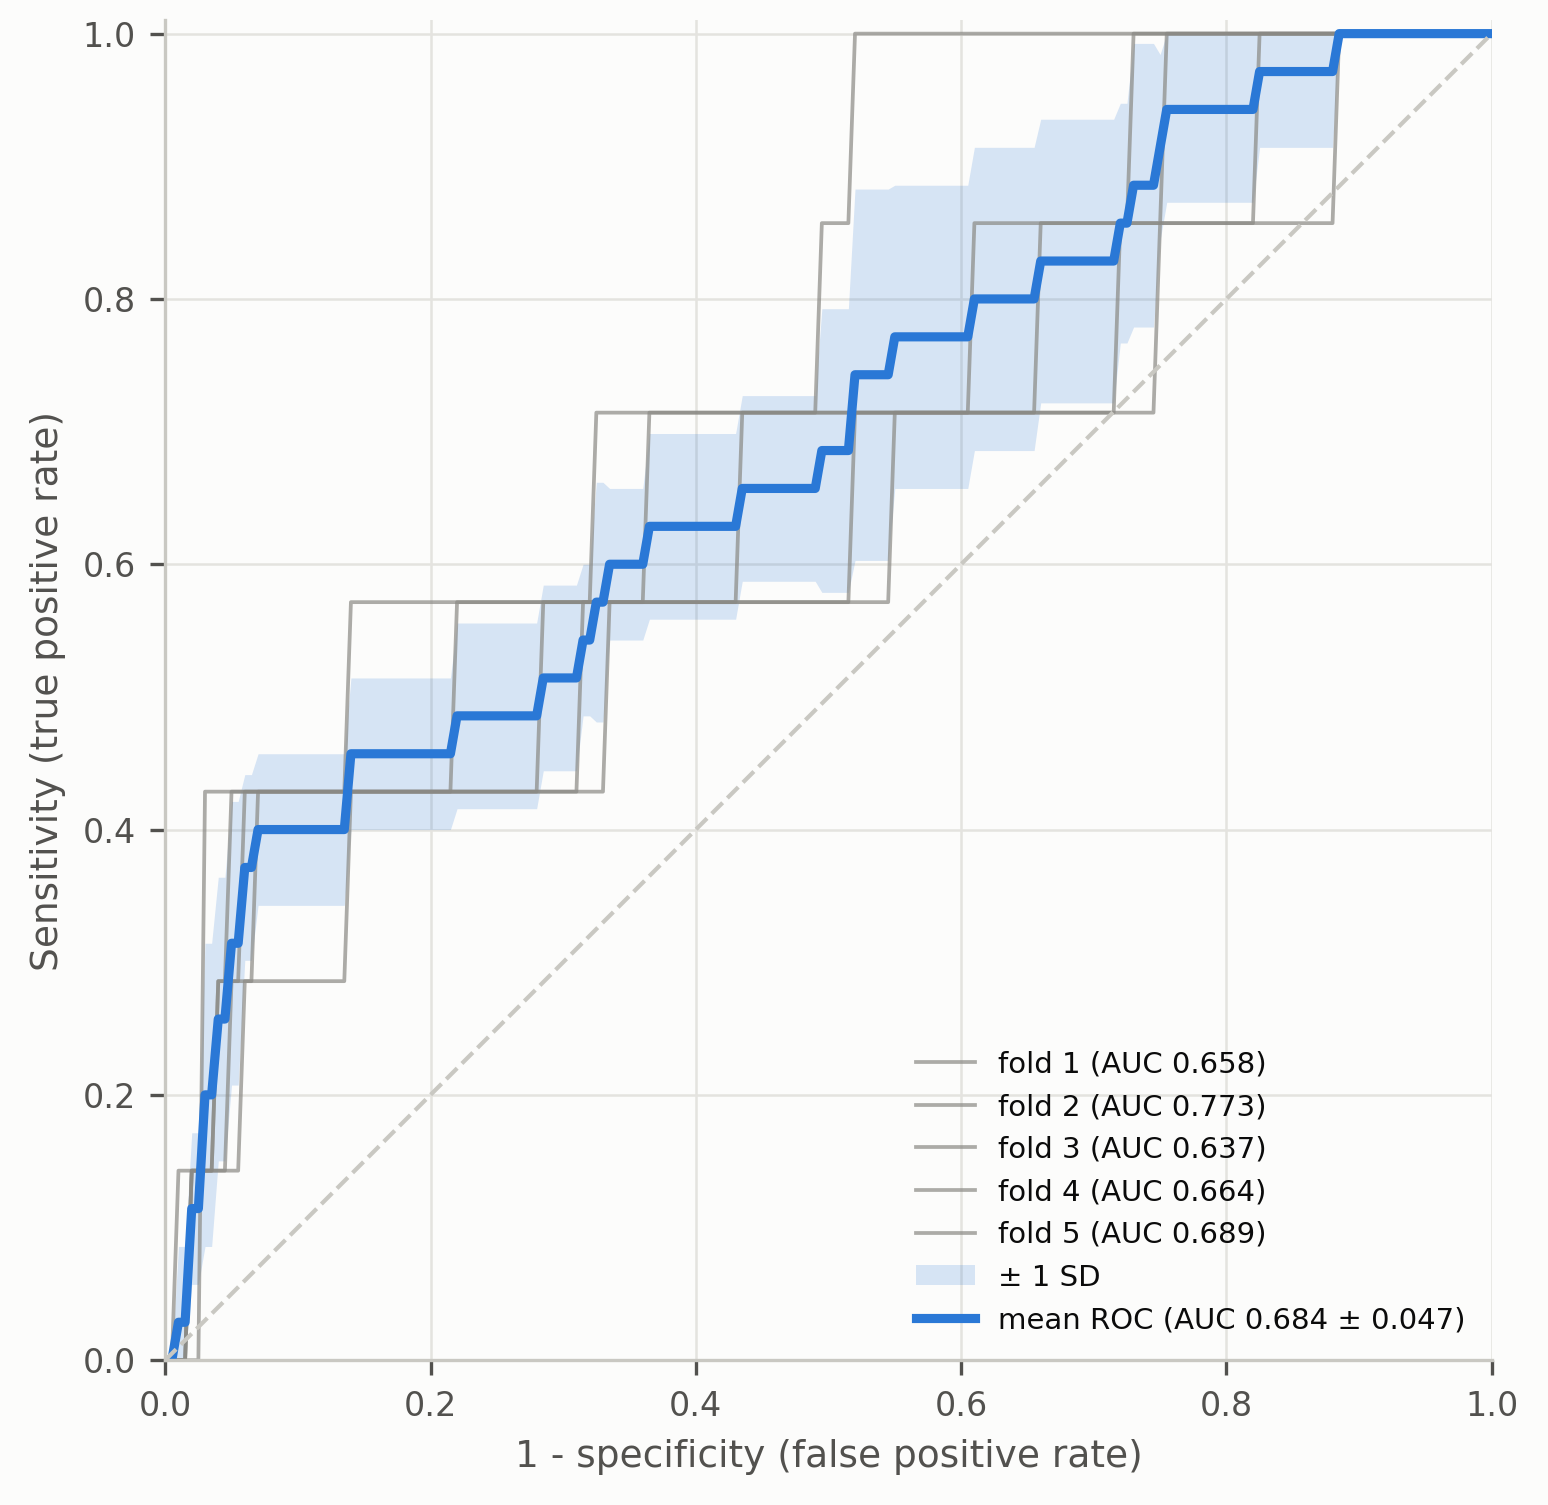
\includegraphics[width=0.48\textwidth]{roc_cv_folds_DM_clean.png}\hfill
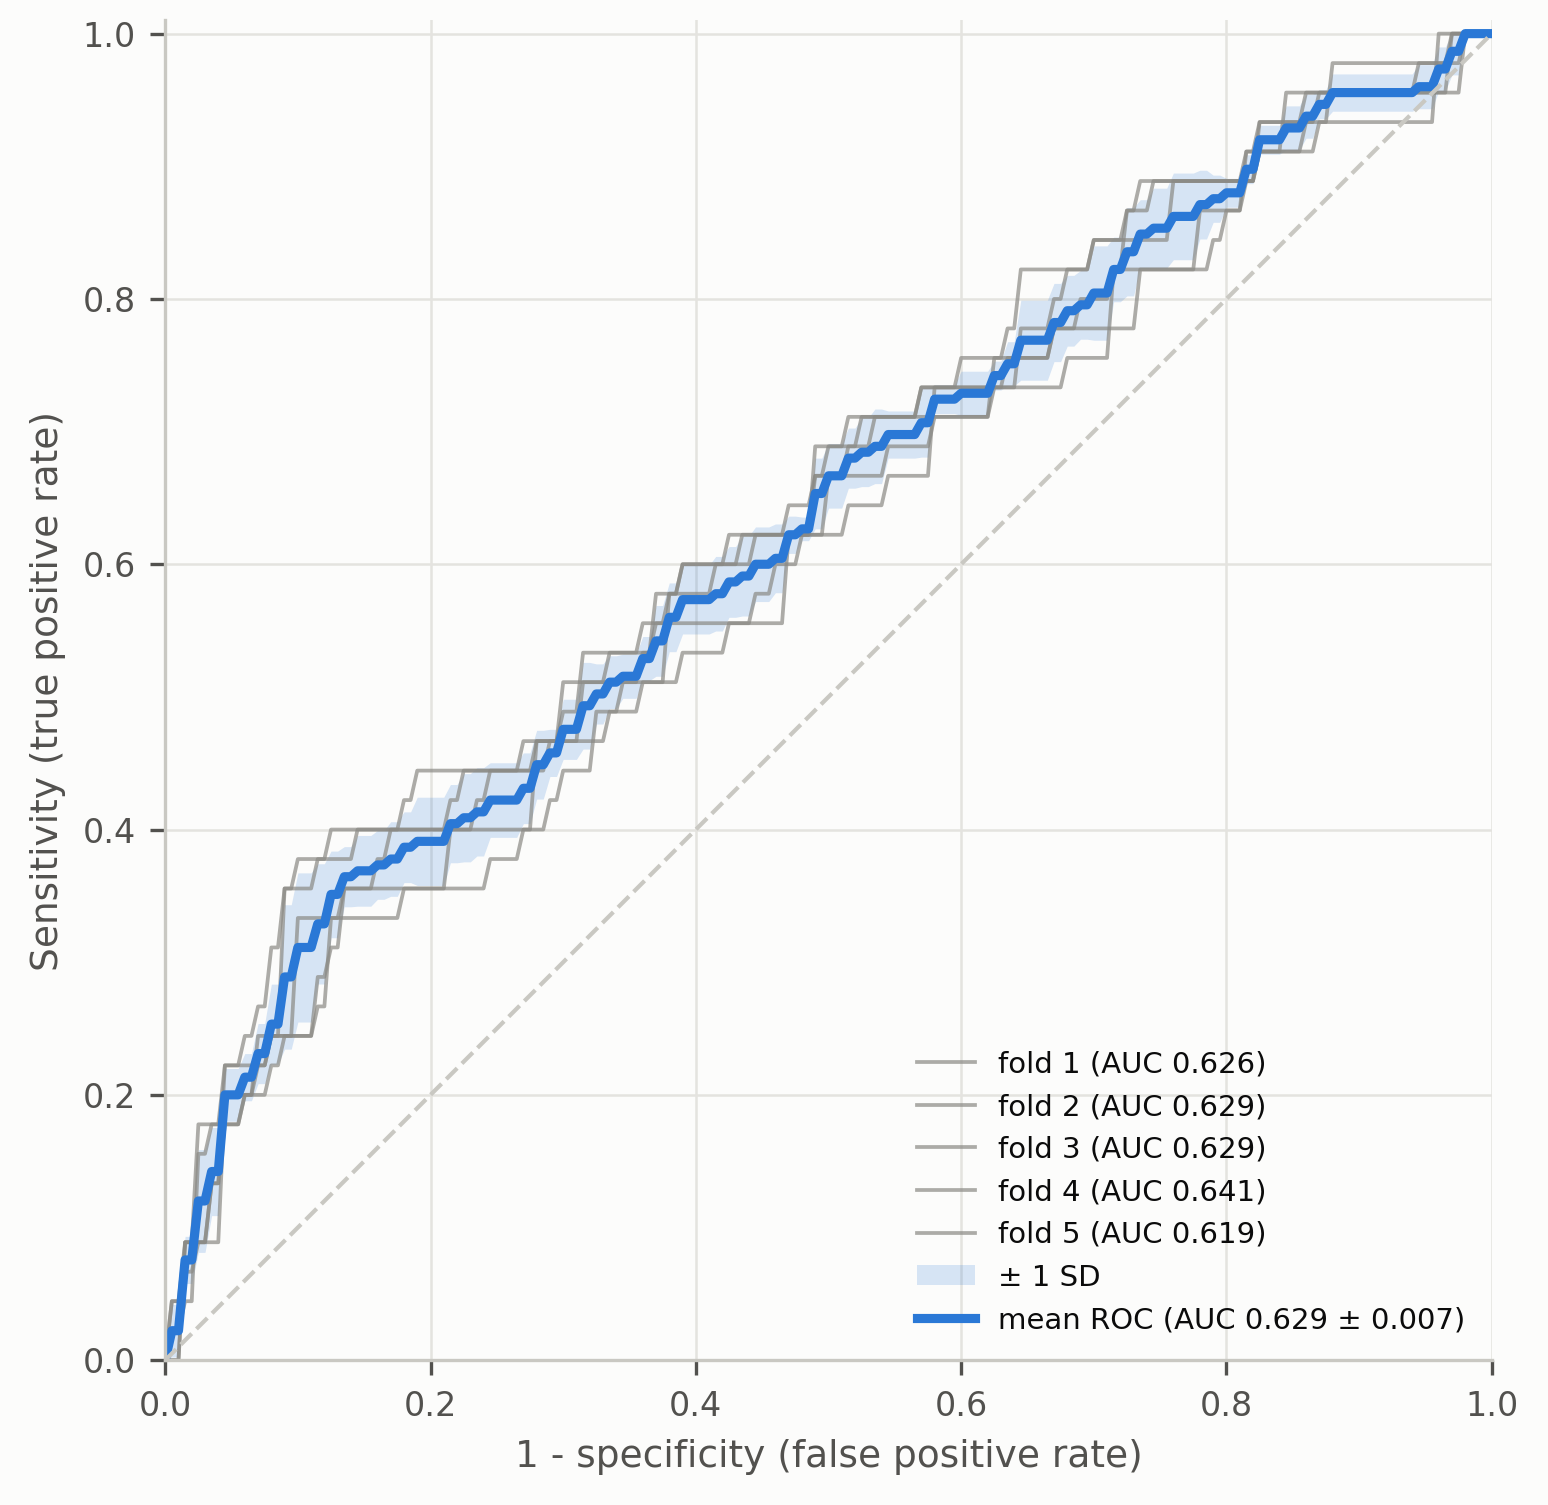
\includegraphics[width=0.48\textwidth]{roc_cv_folds_OS_clean.png}
\caption{External ROC curves of the five fold models of the configuration chosen in cross-validation, with mean curve and $\pm1$ standard deviation, for distant metastasis (left) and overall survival (right).}\label{fig:foldsDMOS}
\end{figure}

%% =========================================================================================
\section{Reproducibility checklist}

\begin{table}[!htb]
\centering\small
\caption{Reproducibility items identified by Mateus et al.\ and how they are addressed in this study.}\label{tab:checklist}
\begin{tabular}{@{}p{0.3\textwidth}p{0.62\textwidth}@{}}
\toprule
Item & This study \\
\midrule
Public data & Head-Neck-PET-CT and HN1 (The Cancer Imaging Archive) \\
Data split & 5-fold stratified CV and cohort split (HGJ+CHUS / HMR+CHUM); split files stored \\
Endpoint definition & binary horizons (2 years for LR and DM, 4 years for OS); patients censored before the horizon excluded \\
Image pre-processing & fully specified (Table~\ref{tab:preproc}); cached and versioned \\
Random seeds & fixed (42--44); deterministic pipeline \\
Model selection & lowest validation loss (primary) and Mateus et al.\ rule (sensitivity) \\
Software environment & package versions in \texttt{requirements.txt}; setup check script \\
Code & complete pipeline, checkpoints and inference tool released \\
Trained models & self-contained checkpoints (weights, features, scaler, encoder, threshold, topology) \\
\botrule
\end{tabular}
\end{table}

\end{document}
